\chapter{Modelos implementados}
\label{chapter:modelos}

En este capítulo vamos a repasar qué modelos he implementado y cómo funcionan cada uno de ellos. Primero se hará una revisión teórica de los modelos y posteriormente un análisis breve del código explicando las particularidades de las implementaciones.

\section{Algoritmos de ensamblaje}

Los algoritmos que he implementado pertenecen a una familia concreta de algoritmos de detección de anomalías denominados como algoritmos de ensamblaje o ``Ensemble Algorithms'' en inglés. Estos algoritmos son lo equivalente a los meta-algoritmos pero destinados a la detección de anomalías. Para dar una mejor definición de qué son los algoritmos de ensamblaje vamos a introducir una clasificación de los mismos para dar las categorías que entran dentro de esta definición.

\begin{itemize}
	\item Algoritmos de ensamblaje secuenciales: En este tipo de algoritmos tenemos un algoritmos base o un conjunto de algoritmos base que se aplican de forma secuencial, de forma que las primeras ejecuciones se ven usadas o modificadas por ejecuciones futuras de algoritmos. Finalmente el resultado puede ser una combinación ponderada de las valoraciones de los algoritmos o el resultado del último de ellos.
	
	
	\begin{algorithm}[H]{\textbf{Ensamblaje secuencial:}}
		\SetAlgoLined
		
		\textbf{Entrada: } Conjunto de datos $\mathcal{D}$, Algoritmos base $\mathcal{A}_1 , ... , \mathcal{A}_r$
		
		j=1
		
		\Repeat{fin}{
			Tomamos el algoritmo $\mathcal{A}_j$ según los resultados anteriores
			
			Tomamos el conjunto de datos modificado $f_j (\mathcal{D})$ de anteriores ejecuciones
			
			Ejecutamos el algoritmo $\mathcal{A}_j$ sobre $f_j (\mathcal{D})$
			
			j=j+1
			
		}
	
		\KwResult{Combinación de los resultados}
	\end{algorithm}
	\item Algoritmos de ensamblaje independientes: En este caso se emplean o bien diferentes instancias del mismo algoritmo o bien diferentes porciones de los datos que se emplearán de forma distinta. Se puede variar la instanciación por ejemplo dependiendo del subespacio sobre el que queramos ejecutarlo o dependiendo de las características de una porción concreta de los datos.
	
	\begin{algorithm}[H]{\textbf{Ensamblaje independiente:}}
		\SetAlgoLined
		
		\textbf{Entrada: } Conjunto de datos $\mathcal{D}$, Algoritmos base $\mathcal{A}_1 , ... , \mathcal{A}_r$
		
		j=1
		
		\Repeat{fin}{
			Tomamos el algoritmo $\mathcal{A}_j$
			
			Creamos el conjunto de datos modificado $f_j (\mathcal{D})$
			
			Ejecutamos el algoritmo $\mathcal{A}_j$ sobre $f_j (\mathcal{D})$
			
			j=j+1
			
		}
		
		\KwResult{Combinación de los resultados}
	\end{algorithm}
\end{itemize}

\section{Mahalanobis Kernel}

Este algoritmo está englobado dentro de la categoría de algoritmos basados en dependencia. Esta clase de algoritmos intenta estudiar las dependencias que existen entre atributos para así poder detectar las instancias u objetos que no tienen estas dependencias y marcarlos como anomalías.

Si intentamos visualizar esta dependencia entre atributos de forma gráfica lo que observaríamos es que los datos están alineados o posicionados en hiperplanos lineales o no lineales de la siguiente forma:

\begin{figure}[H]
	\centering
	\label{hiperplano}
	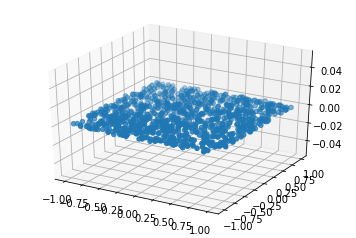
\includegraphics[scale=0.8]{imagenes/hiperplano}
	\caption{Hiperplano}
\end{figure}

Esta figura es un ejemplo clásico de estudio de algoritmos como por ejemplo PCA (algoritmo que quedaría dentro de esta categoría).

\begin{figure}[H]
	\centering
	\label{hiperboloide}
	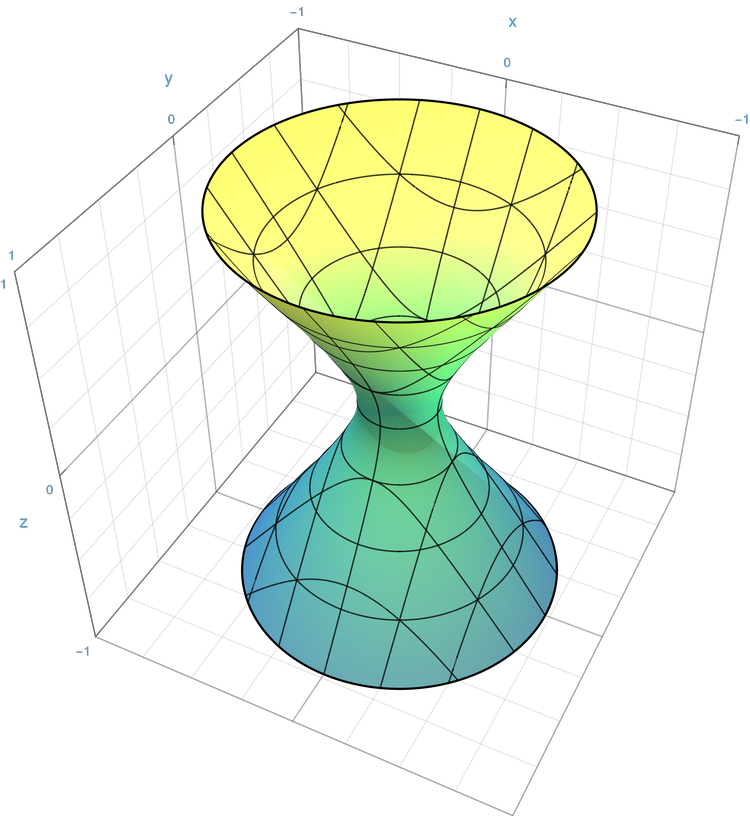
\includegraphics[scale=2.5]{imagenes/hiperboloide}
	\caption{Hiperboloide \href{https://commons.wikimedia.org/wiki/File:Circular_Hyperboloid_Of_One_Sheet_Quadric.png}{Wikimedia}}
\end{figure}

En este caso tenemos el ejemplo de un hiperboloide que no tiene una dependencia lineal, si no que presenta una dependencia de tipo cuadrático.

El método de Mahalanobis Kernel puede ser visto como una modificación de PCA. PCA básicamente dispone de dos pasos:

\begin{enumerate}
	\item Determinar un sistema ortogonal de direcciones principales y proyectar los datos sobre este sistema.
	\item Calcular la distancia entre el punto original y la proyección como su puntuación de anomalía.
\end{enumerate}

El método Mahalanobis Kernel intenta tener este mismo comportamiento en dos pasos y que ahora veremos. El algoritmo PCA es muy útil cuando los datos tienen atributos relacionados en un hiperplano, mientras que Mahalanobis Kernel funciona mejor cuando los datos están relacionados en formas más complejas como el hiperboloide que hemos enseñado. La elección de este algoritmo en vez de PCA recae en el hecho de que PCA es un algoritmo clásico y el escenario en el que mejor funciona (hiperplano) es más restrictivo que el que nos ofrece Mahalanobis Kernel con un abanico de figuras más amplio.

Vamos a describir el funcionamiento del algoritmo, pero primero vamos a introducir notación. Vamos a llamar $D$ a la matriz de datos que está centrada en la media y que tiene dimensiones $n\times d$, es decir, tenemos $n$ instancias u objetos de dimensionalidad $d$.

\begin{algorithm}{\textbf{Mahalanobis Kernel}}
	\caption{Mahalanobis Kernel}
	\label{mahalanobis_kernel}
	\KwIn{$D$}
	
	$S = DD^T$.
	
	$S = Q\Delta^2 Q^T$.
	
	Almacenamos los vectores propios columna no negativos de $Q\Delta$ en una matriz $D'$
	
	Normalizamos $D'$ para que tenga media $0$ y varianza $1$.
	
	$vector\_media = media(D')$
	
	$puntuaciones = []$
	
	\ForEach{fila en D'}{
		$score = distancia(vector\_media , fila)$
		
		$puntuaciones = [puntuaciones, score]$
	}
	\KwOut{puntuaciones}
\end{algorithm}

El algoritmo comienza con la matriz de datos $D$. Se obtiene la matriz simétrica $S$ y se hace la descomposición en valores singulares. 

Con este modelo tenemos las dos fases que teníamos en PCA. Primero obtenemos una matriz $D'$ de los datos proyectados y transformados para posteriormente reportar la puntuación de anomalía como una distancia.

Veamos ahora la implementación en Python.

\begin{lstlisting}[language=Python]
def runMethod(self):
	'''
	@brief Function that executes the Kernel Mahalanobis method. The results are
	stored on the variable self.scores
	@param self
	'''
	''' Compute the S matrix of the algorithm'''
	S = np.dot(self.dataset, self.dataset.T)
	''' Now we diagonalize it'''
	Q,delta_sq,Qt = np.linalg.svd(S)
	del S
	del Qt
	''' Obtain delta as matrix'''
	delta = np.matrix(np.diag(np.sqrt(delta_sq)))
	del delta_sq
	Q = np.matrix(Q)
	''' Compute de D' matrix and normalize it'''
	Dprime = np.dot(Q,delta)
	del Q
	del delta
	Dp_std = scale(Dprime, axis=1)
	del Dprime
	''' We compute its mean on the rows to compute the deviation as the score'''
	mean = Dp_std.mean(axis=0)
	self.outlier_score=[]
	''' The score is the euclidean distance to the mean'''
	for i in range(len(Dp_std)):
		self.outlier_score.append(np.linalg.norm(mean-Dp_std[i])**2)
	self.outlier_score = np.array(self.outlier_score)
	self.calculations_done=True
\end{lstlisting}

La implementación del algoritmo se ha realizado en Python como el resto del proyecto y posteriormente se explicará en detalle cómo se ha organizado.

El algoritmo basa su implementación en la librería NumPy.

\section{TRINITY}

Este algoritmo es del segundo tipo que vimos al principio cuando hicimos una categorización de los algoritmos de ensamblaje, en concreto el algoritmo hace una combinación de tres componentes distintos. La intención de hacer esta composición de modelos es intentar obtener todos los tipos de anomalías que se puedan del conjunto y que reciban una puntuación acorde. La teoría nos dice que esta combinación de modelos nos va a proveer de un resultado más robusto que el uso de modelos aislados como discutiremos en la sección de resultados.

En concreto este algoritmo consta de tres componentes distintos:

\begin{itemize}
	\item Componente basado en distancias: este componente consta de un algoritmo que base u comportamiento en técnicas de agrupamiento o valoración por distancias como por ejemplo es el método clásico KNN. Este método lo que hace es tomar los k vecinos más cercanos y colocar como puntaje de anomalía para esa instancia como la suma de estas distancias. De esta forma los puntos que más alejados estén del resto sumarán una mayor distancia y por tanto serán más anómalos. En concreto este modelo se ha utilizado con el valor $k=5$ y con una técnica de subsampling. La técnica de subsampling consiste en no utilizar todo el conjunto de datos en el algoritmo, si no particionarlo y utilizar una pequeña muestra repitiendo este proceso y haciendo la media de las ejecuciones. De esta forma conseguimos una reducción de la varianza. Esto conlleva algunas ventajas como discutimos en la sección de sesgo y varianza anteriormente. En concreto la técnica toma 1000 particiones, ejecuta el algoritmo sobre ellas y hace la media.
	\item Componente basado en dependencia: este componente toma un algoritmo como el que hemos implementado (Mahalanobis Kernel). En este componente vamos a intentar detectar las anomalías que corresponden a datos que no siguen las relaciones entre atributos que sí tienen el resto de los objetos. Para ello he utilizado en este componente el algoritmo Mahalanobis Kernel que ya hemos explicado anteriormente incorporando la técnica de subsampling.
	\item Componente basado en densidad en subespacios: en este componente vamos a incorporar un modelo que intente buscar anomalías que lo sean en base a la densidad que tienen en alguno de los subespacios de los datos. Este hecho no nos debe ser ajeno pues es la segunda de las definiciones que hemos visto de anomalía y que hacía referencia a la función de densidad y los subespacios incorrelados y correlados. En concreto para este componente he utilizado el algoritmo IForest o Isolation Forest. Este algoritmo lo que hace es tomar de forma aleatoria un atributo y se van particionando los valores del mismo en una estructura de árbol, es decir, dividimos los datos en aquellos con un valor superior al marcado para el atributo y con un valor menor. De esta forma podemos medir cuántos pasos o lo que es lo mismo qué profundidad ha alcanzado nuestro árbol hasta llegar a dividir un objeto del resto de los datos. Este algoritmo también incorpora la técnica de subsampling.
\end{itemize}

Por último con esto hemos obtenido tres vectores o listas con la puntuación que cada componente nos ha arrojado para cada instancia. Para hacerlos comparables lo que debemos hacer es estandarizar los datos a media cero y varianza unitaria. Finalmente se realiza la media de los tres vectores de puntaje siendo esta la puntuación final devuelta por TRINITY.

Veamos la implementación de este algoritmo:

\begin{lstlisting}[language=Python]
def distanceBased(self):
	'''
	@brief Function that implements the distance based component
	@param self
	@return It returns the vector with the scores of the instances
	'''
	''' Initialize the scores'''
	scores = np.array([0]*len(self.dataset)).astype(float)
	for i in range(self.num_iter):
		knn = KNN(n_neighbors=5, contamination=self.contamination)
		''' Number in the interval [50, 1000]'''
		subsample_size = np.random.randint(50, 1001)
		sample = []
		if subsample_size>=len(self.dataset):
			sample = list(range(len(self.dataset)))
		else:
			''' Take the sample and train the model'''
			sample = np.random.choice(len(self.dataset), size=subsample_size, replace=False)
		knn.fit(self.dataset[sample])
		''' Update the score to compute the mean'''
		scores[sample]+=knn.decision_scores_
	''' Return the mean'''
	scores = scores/self.num_iter
	scores = scale(scores)
	return scores

def dependencyBased(self):
	'''
	@brief Function that implements the dependency based component
	@param self
	@return It returns the vector with the scores of the instances
	'''
	''' Initialize the scores'''
	scores = np.array([0]*len(self.dataset)).astype(float)
	for i in range(self.num_iter):
		kernel_mahalanobis = KernelMahalanobis(contamination=self.contamination)
		''' Number in the interval [50, 1000]'''
		subsample_size = np.random.randint(50, 1001)
		sample = []
		if subsample_size>=len(self.dataset):
			sample = list(range(len(self.dataset)))
		else:
			''' Take the sample and train the model'''
			sample = np.random.choice(len(self.dataset), size=subsample_size, replace=False)
		kernel_mahalanobis.fit(self.dataset[sample])
		''' Update the score to compute the mean'''
		scores[sample]+=kernel_mahalanobis.outlier_score
	''' Return the mean'''
	scores = scores/self.num_iter
	scores = scale(scores)
	return scores

def densityBased(self):
	'''
	@brief Function that implements the dependency based component
	@param self
	@return It returns the vector with the scores of the instances
	'''
	''' Initialize the scores'''
	scores = np.array([0]*len(self.dataset)).astype(float)
	for i in range(self.num_iter):
		iforest = IForest(contamination=self.contamination, behaviour="new")
		''' Number in the interval [50, 1000]'''
		subsample_size = np.random.randint(50, 1001)
		sample = []
		if subsample_size>=len(self.dataset):
			sample = list(range(len(self.dataset)))
		else:
			''' Take the sample and train the model'''
			sample = np.random.choice(len(self.dataset), size=subsample_size, replace=False)
		iforest.fit(self.dataset[sample])
		''' Update the score to compute the mean'''
		scores[sample]+=iforest.decision_scores_
	''' Return the mean'''
	scores = scores/self.num_iter
	scores = scale(scores)
	return scores

def runMethod(self):
	'''
	@brief This function is the actual implementation of TRINITY
	@param self
	'''
	''' Distance module'''
	if self.verbose:
		print("Obtaining scores with the distance module")
	distance_based = self.distanceBased()
	''' dependency module'''
	if self.verbose:
		print("Obtaining scores with the dependency module")
	dependency_based = self.dependencyBased()
	''' Density module'''
	if self.verbose:
		print("Obtaining scores with the density module")
	density_based = self.densityBased()
	
	''' Compute the mean of the three modules'''
	self.outlier_score=(distance_based + dependency_based + density_based)/3
	self.calculations_done=True
\end{lstlisting}

Todos los módulos tienen una función parecida. En primer lugar se inicializan las puntuaciones y se repite el mismo proceso de cálculo 100 veces. Se inicializa el modelo y se ajusta con una muestra de tamaño en el intervalo $[50,1000]$. Por último se hace la media de todos los cálculos y se estandarizan con la librería Sklearn.

En la función principal ``runMethod'' se ejecutan los tres módulos y se hace la media de las puntuaciones.